\documentclass[conference]{IEEEtran}
\IEEEoverridecommandlockouts

\usepackage[T1]{fontenc}
\usepackage[utf8]{inputenc}
\usepackage{cite}
\usepackage{amsmath,amssymb,amsfonts,bm}
\usepackage{graphicx}
\usepackage{booktabs}
\usepackage{url}
\usepackage{xcolor}
\usepackage[hidelinks]{hyperref}

\graphicspath{{figures/}}

\begin{document}

\title{Trajectory Calibration for Agentic Digital Twins\
Requires Measured Telemetry:\
A Provenance and Leakage Audit on PHMForge}

\author{\IEEEauthorblockN{Umberto Altieri}
\IEEEauthorblockA{\textit{Independent Researcher}\
\texttt{altieriumb7@gmail.com}}}

\maketitle

\begin{abstract}
Agentic Digital Twins (ADTs) delegate diagnostic and maintenance decisions to
tool-augmented Large Language Models, so knowing when such an agent is about to
fail is a safety requirement rather than a convenience. A natural proposal, and
the one we pursued in an earlier version of this work, is to predict trajectory
failure from a diagnostic feature vector combining token-level uncertainty,
verbalized confidence, and Model Context Protocol (MCP) execution telemetry. We
report here that our own initial result---an $83\%$ reduction in expected
operational cost and a feature ranking in which logprob variance dominated---did
not survive an audit of where its features came from. We identify six defects
that we believe generalise well beyond this study. First, the token-level
features were \emph{synthesised}: the logging layer fabricated per-token
logprobs from a hard-coded confidence constant, and the $203{,}107$ recorded
values fit the generator's $\mathcal{N}(-0.40, 0.225^2)$ law
(observed $-0.4030 \pm 0.2182$). Second, verbalized confidence was never
elicited from any model; $162$ of $167$ trajectories carry an identical
fallback value, and because it was parsed once per trajectory rather than per
step, its gradient is zero by construction. Third, the tool-error rate---the one
signal that looks like genuine telemetry---is never read from Model Context
Protocol responses, but inferred by substring-matching the observation text.
Fourth, the harness writes a terminal observation reading literally ``Task
finished successfully'' or ``Task failed'', so any feature derived from
observation text reads the label. Fifth, the telemetry was never observed at
all: it is re-derived by parsing run logs, and the reconstruction inflates the
step sequence every structural feature is computed over---the single-use
\texttt{Finish} action appears $866$ times across $167$ trajectories. Taken
together, no feature in this corpus is a measurement. A sixth defect concerns
the target rather than the features: on $30$ of the $75$ scenarios the tool layer
fabricates the analytical outcome---returning ground truth plus fixed-seed noise
tuned to pass the grader---so a success there records tool orchestration, not
prognostic accuracy. We turn that split into a stratified design rather than
repairing it. Re-running the study with scenario-grouped
cross-validation, bootstrap intervals, and permutation tests, no
leakage-controlled signal set separates success from failure above chance once
the six comparisons are corrected for (best AUROC $0.566$, $95\%$ CI
$[0.479, 0.650]$, $p = 0.074$), whereas the contaminated variant reaches
$0.881$ at $p < 0.001$. Under a
cost model, the optimal selective policy degenerates to always-abstain, a
trivial baseline the original study never compared against.

We then repaired the instrumentation and re-collected the benchmark on three
open-weights backbones, which required leaving the managed inference gateway
entirely: it refuses to return logprobs on every open-weights model it hosts, so
token-level uncertainty is unobservable there --- an awkward fact for a setting
whose deployments are the least able to use a commercial API. On the re-collected
corpus the pooled answer is close to null, and the stratified one is not: the
measured signals predict failure on the scenarios whose tools genuinely compute
an outcome, and not on those whose outcome is fabricated. Holding the backbone
fixed, token-level uncertainty predicts failure on the smaller model and not the
larger, and permutation importance attributes essentially all of it to the
entropy of the first two steps rather than to variance over the whole
trajectory --- which would support abstaining early rather than after the fact.
We release a provenance gate that reproduces every finding, fails closed on the
original corpus, and detects the two failure modes that defeated us on the
corrected one, and argue that feature provenance belongs in agentic-calibration
papers as a first-class experimental artifact.
\end{abstract}

\begin{IEEEkeywords}
Agentic Digital Twins, predictive maintenance, uncertainty quantification,
data leakage, selective prediction, Model Context Protocol, negative results.
\end{IEEEkeywords}

\section{Introduction}

Industrial Digital Twins are moving from passive simulation toward autonomous
management, in which an LLM agent receives a high-level request---estimate the
remaining useful life of a turbofan, decide whether a bearing warrants
intervention---and satisfies it by orchestrating diagnostic tools over the
Model Context Protocol (MCP)~\cite{mcp}. Benchmarks such as
PHMForge~\cite{phmforge} and AssetOpsBench~\cite{assetops} show that even strong
backbones complete only around two thirds of such tasks. Because an unnoticed
prognostic failure on safety-critical plant is far more costly than a deferred
decision, an ADT that can recognise its own unreliable trajectories and abstain
is worth more than one that is merely more accurate.

This motivates \emph{trajectory calibration}: predicting, from signals observable
during execution, whether an agent's run will succeed. The signals usually
proposed fall into three families---token-level uncertainty derived from
generation logprobs~\cite{kadavath}, verbalized self-reported
confidence~\cite{xiong}, and execution telemetry such as tool-call errors and
repeated actions~\cite{calvert}.

An earlier version of this paper reported that a hybrid of these signals
predicted PHMForge failures well enough to cut expected operational cost by
$83\%$, and that logprob variance ($30.0\%$) and MCP error ratio ($28.7\%$)
dominated the feature ranking while verbalized confidence contributed under
$4\%$. This paper retracts those claims and explains why. The headline numbers
were arithmetically reproducible but scientifically empty: two of the three
signal families were never measured, and the apparent predictive power came
from the grading harness leaking its verdict into the feature space.

We make four contributions.
\begin{enumerate}
  \item A \textbf{provenance audit} that identifies six concrete defects in a
  plausible-looking agentic-telemetry pipeline, each detectable by a cheap test
  we describe (Sec.~\ref{sec:defects}), together with a released gate that
  automates those tests and fails closed.
  \item A \textbf{leakage-controlled re-evaluation} with scenario-grouped
  cross-validation, bootstrap confidence intervals, and permutation tests,
  showing that no admissible signal set beats chance on this corpus
  (Sec.~\ref{sec:results}).
  \item A \textbf{corrected cost analysis} showing that the original $83\%$
  saving was measured against the wrong baseline, and that the cost-optimal
  policy here is to abstain on everything (Sec.~\ref{sec:cost}).
  \item A \textbf{reporting checklist} for agentic-calibration studies
  (Sec.~\ref{sec:checklist}), with the audit harness released for reuse.
\end{enumerate}

We stress that the defects are not exotic. Synthesising a missing feature to
keep a pipeline running, defaulting an unparsed field, and letting a grader's
message flow into a logged trace are all ordinary engineering decisions. What
makes them dangerous is that each one produces a feature column that looks
numerically healthy and passes every check short of asking where the numbers
came from.

\section{Background and Related Work}

\textbf{Agentic benchmarks for maintenance.} PHMForge~\cite{phmforge} supplies
expert-curated prognostics and health-management scenarios---RUL prediction,
fault classification, engine health analysis, cost--benefit and safety
evaluation---exposed through MCP-native, algorithm-grounded tools, and reports
that even leading configurations top out near $68\%$ task completion.
AssetOpsBench~\cite{assetops} targets the same operational domain. Both use
ReAct-style~\cite{react} agents that interleave thought, action, and
observation.

\textbf{Uncertainty quantification for LLM agents.} Calibration asks that stated
confidence match empirical correctness~\cite{guo,naeini}. For single-turn
generation, token logprobs carry real signal~\cite{kadavath}, whereas verbalized
confidence is typically overconfident and weakly discriminative~\cite{xiong}.
For \emph{agents}, CalVerT~\cite{calvert} augments agent state with calibrated
self-confidence and verifier telemetry on knowledge-intensive tasks. Our earlier
version described a logistic model on MCP error rates as ``CalVerT''; that was a
misattribution, and we correct it here---CalVerT is a different method on a
different task, and the model we evaluated is our own.

\textbf{Selective prediction.} Abstention has a long formal
treatment~\cite{elyaniv,geifman}: a selective classifier trades coverage for
risk, and the standard evaluation is a risk--coverage curve. Two policies bound
any such curve---executing everything and abstaining on everything---and a
selective method is only interesting if it beats both under the operative cost
model. Sec.~\ref{sec:cost} shows the original study omitted the second bound.

\textbf{Leakage.} Kapoor and Narayanan~\cite{kapoor} catalogue leakage as a
leading cause of irreproducibility in ML-based science, with the
illegitimate-feature variety---a feature that encodes the target---the most
common. The defect in Sec.~\ref{sec:leak} is a textbook instance arising from
agent-harness design rather than from dataset construction.

\section{Study Setup}

We evaluate seven backbones---\texttt{granite-4-h-small},
\texttt{llama-3.3-70b}, \texttt{llama-4-maverick}, \texttt{mistral-medium-2505},
\texttt{mistral-small-24b}, \texttt{gpt-oss-120b}, and
\texttt{gpt-4o-mini}---on $25$ PHMForge scenarios spanning RUL prediction, fault
diagnosis, engine health, cost--benefit, and safety tasks. Agents are ReActXen
ReAct loops with MCP tool access. After discarding empty logs this yields
$n = 167$ trajectories with an overall Pass@1 of $0.539$.

A trajectory is a sequence
$\tau = (s_0, a_0, o_0, \ldots, s_T)$ of thought, action, and observation steps.
Each logged step records the action and its input, the MCP calls it issued with
their status codes, a per-token logprob array, a verbalized confidence, and the
task-success label. Our target is binary trajectory success, and the
quantity of interest is whether any function of $\tau$ predicts it.

\begin{figure*}[t]
\centering
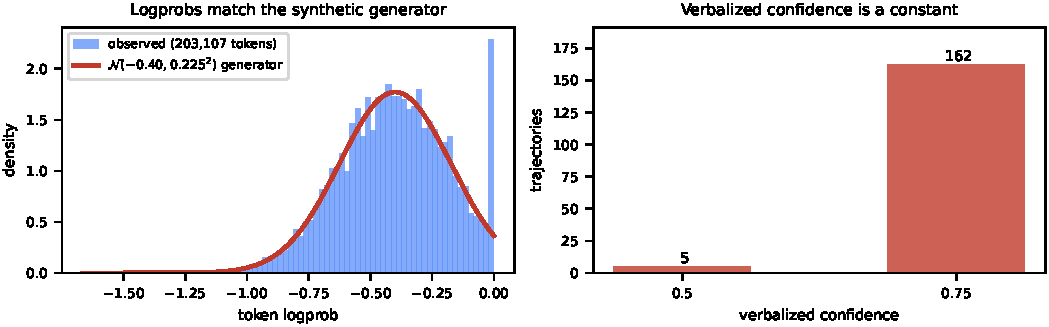
\includegraphics[width=\textwidth]{fig2_provenance.pdf}
\caption{Provenance evidence. \textbf{Left:} the empirical distribution of all
$203{,}107$ logged token logprobs against the density of the logging layer's
own synthetic generator at its default confidence of $0.75$. The fit is exact
(observed $-0.4030 \pm 0.2182$ against a predicted $-0.4000 \pm 0.2250$); the
spike at zero is the generator's clipping. \textbf{Right:} verbalized
confidence takes one value on $162$ of $167$ trajectories. Neither family was
measured from a model.}
\label{fig:provenance}
\end{figure*}

\section{Six Provenance Defects}
\label{sec:defects}

\subsection{Token-level uncertainty was synthesised}

No component ever requests logprobs. The string \texttt{logprob} does not occur
anywhere in the inference client: neither the watsonx generation parameters nor
the OpenAI-compatible request body asks for them, and no response object
carries them. The ReAct agent's \texttt{prompt\_agent} does contain code that
looks for a \texttt{token\_logprobs} key, so the receiving half of the chain was
written; the producing half never was.

The gap is filled downstream. The telemetry logger, finding the field empty,
calls a helper documented as generating ``realistic token-level logprobs.''
That helper draws each token's value from $\mathcal{N}(\mu, \sigma^2)$ with
\begin{equation}
\mu = -0.1 - 1.2\,(1 - c), \qquad
\sigma = 0.15 + 0.3\,(1 - c),
\end{equation}
where $c$ is the trajectory's verbalized confidence. Since $c$ is itself a
constant $0.75$ (Sec.~\ref{sec:verbal}), every logprob in the corpus is an
i.i.d.\ draw from a single fixed law, independent of the backbone, the scenario,
and the outcome.

The test is one line: compare the empirical moments of the logged values against
what the generator would produce. Across $203{,}107$ tokens we observe
$-0.4030 \pm 0.2182$ against a predicted $-0.4000 \pm 0.2250$
(Fig.~\ref{fig:provenance}, left). The match is exact, and no provider-returned
logprobs survive anywhere in the corpus.

The defect is worse than a missing request. We patched the client to ask for
logprobs and probed the hosting service directly: for all five open-weights
backbones it answers \texttt{parameter `logprobs' is no longer supported for
this model and is ignored}, on both the \texttt{generate} and \texttt{chat}
endpoints. The rejection is a warning, not an error, so the call succeeds and
the field is simply absent. Token-level uncertainty was therefore not merely
unrequested but \emph{unobtainable} on this stack, and the fallback made the
impossibility invisible. Of the seven backbones only the commercial
\texttt{gpt-4o-mini} returns logprobs at all --- a point we return to in
Sec.~\ref{sec:limitations}, because it bears directly on whether the study can
be run on the models an industrial deployment could actually host.

Consequently \emph{early entropy} and \emph{logprob variance}---which our
earlier feature ranking placed first and third, together carrying $52.7\%$ of
the attributed importance---are functions of pseudorandom noise. Table~\ref{tab:main}
confirms it empirically: a model given only these two features scores AUROC
$0.444$ ($p = 0.889$), indistinguishable from chance in the direction one would
expect of pure noise.

\subsection{Verbalized confidence was never elicited}
\label{sec:verbal}

The confidence parser scans the agent's text for an explicit percentage and,
failing that, may query a callback; when both miss it returns a literal
\texttt{0.75}, annotated as a ``realistic baseline default.'' Every path except
that default is dead in this corpus. Of $167$ trajectories, $162$ carry exactly
$0.75$ and $5$ carry $0.5$, the latter being a distinct fallback triggered on
degenerate logs (Fig.~\ref{fig:provenance}, right).

This invalidates the original claim that verbalized confidence is
uninformative. The claim happens to agree with the literature~\cite{xiong}, but
we did not test it: a constant column carries no information by construction,
and its $3.98\%$ attributed importance was noise admitted by the impurity
criterion. The residual AUROC of $0.532$ in Table~\ref{tab:main} is likewise an
artifact---all five $0.5$-valued trajectories happen to be failures, so the
column is weakly separating for a reason that has nothing to do with a model
expressing doubt.

A second, structural error compounds it. The logger parses confidence
\emph{once} per trajectory, from the final answer, and then writes that single
value into every step record. The confidence gradient $\nabla\text{Conf}$---one
of the six declared dimensions---is therefore the slope of a repeated
constant, and is zero by construction on all $167$ trajectories (exactly $0$ on
$71$; $|\text{slope}| < 10^{-16}$ from \texttt{polyfit} rounding on the rest).
It was never capable of measuring anything. A confidence gradient requires
per-step elicitation, which the original prompt never requested.

Note also the interaction: because the synthetic logprob generator is
parameterised by $c$, a defect in the confidence parser silently propagates into
the token features. Fabricated inputs compose.

\subsection{Tool-error rate is a text heuristic, not telemetry}
\label{sec:mcp}

The MCP error ratio is the feature that most looks like real execution
telemetry, and the one the original ranked second at $28.70\%$. It is not read
from an MCP response. The logger assigns \texttt{status\_code = 400} when the
observation string contains \texttt{"Error"}, \texttt{"Invalid action"}, or
\texttt{"failed"}, and $200$ otherwise. No response metadata is consulted, and
the call site never supplies any. What $\text{Ratio}_{\text{err}}$ measures is
how often those words appear in a tool's printed output---a property of tool
authors' message strings, not of protocol-level execution. A tool that prints
``0 errors found'' on success is recorded as a failure.

Sec.~\ref{sec:results} evaluates an ``execution telemetry'' family, and one
might expect that family at least to rest on measurements. Its error-rate
components come from the same observation text as the leaked verdict, and
Sec.~\ref{sec:recon} shows the remaining components fare no better. The fix is
to record the status the tool server returned, and \texttt{None} otherwise, so
the row is excluded rather than guessed.

\subsection{The telemetry was reconstructed from logs, not observed}
\label{sec:recon}

The sweep script does not instrument the agent. It re-derives trajectories by
parsing ReActXen result logs after the run, and the reconstruction duplicates
steps. Across $167$ trajectories the \texttt{Finish} action---which a ReAct agent
emits once, to terminate---appears $866$ times: $790$ as an intermediate step,
$76$ as a terminal one, absent entirely in $12$ trajectories. $796$ of those
steps carry an empty observation.

Every structural feature is computed over that inflated sequence. Step count,
action-loop ratio, action diversity and termination status therefore describe the
log parser rather than the agent. Combined with the three defects above,
\emph{no feature in this corpus---token, verbalized, error-rate, or
structural---measures the system it purports to describe.}

The defect also removes any trace-shape baseline. We initially read the drop in
terminal-\texttt{Finish} rate between the original corpus and a live capture
($100\%$ against $17\%$) as a regression caused by our own configuration, and
restarted a collection on that basis before establishing that the original figure
counts duplicated steps. Pass@1 survives, because the label comes from the grader
rather than from the reconstruction; nothing about the shape of a trajectory
does.

The general form of this is worth stating plainly: telemetry re-derived from logs
is not telemetry. If the instrumentation does not observe execution as it
happens, the shape of what it reports is a property of the parser.

\subsection{The grader leaks its verdict into observations}
\label{sec:leak}

The harness appends a terminal observation whose text is literally
\texttt{"Task finished successfully"} or \texttt{"Task failed"}. These strings
occur in $70$ of $167$ trajectories and differ in length ($26$ versus $11$
characters), so \emph{any} feature computed over observation text---mean length,
maximum length, a bag-of-words---can recover the label.

The signature is diagnostic. Mean observation length has a univariate AUROC of
only $0.608$, yet a random forest given that single feature reaches an
out-of-fold AUROC of $0.833$. A gap that large between a monotone ranking and a
non-monotone learner means the model is keying on specific values rather than a
trend; here, on the two discrete lengths the grader writes. Removing terminal
and verdict-bearing observations collapses the full model from $0.881$ to
$0.566$ (Table~\ref{tab:main}).

The aggravating factor is structural: $71$ of $167$ trajectories consist of a
single step, so the grader's message is their \emph{only} observation. For
$42.5\%$ of the corpus, observation features are nothing but the label.

\section{Leakage-Controlled Re-evaluation}
\label{sec:results}

\begin{table}[t]
\centering
\caption{Out-of-fold failure prediction on PHMForge ($n=167$ trajectories, scenario-grouped 5-fold CV). Brackets are 95\% bootstrap CIs; $p$ is a label-permutation test against AUROC${=}0.5$.}
\label{tab:main}
\footnotesize
\begin{tabular}{lccc}
\toprule
\textbf{Signal set} & \textbf{AUROC} & \textbf{ECE} & $\bm{p}$ \\
\midrule
Verbalized confidence (raw) & 0.532 [0.507, 0.562] & 0.204 & 0.022 \\
Synthetic token features [RF] & 0.444 [0.348, 0.531] & 0.210 & 0.889 \\
V1 feature vector f(tau) [RF] & 0.590 [0.504, 0.674] & 0.133 & 0.025 \\
MCP error ratio only [LR] & 0.477 [0.388, 0.570] & 0.106 & 0.702 \\
Measured execution telemetry [LR] & 0.580 [0.493, 0.667] & 0.115 & 0.043 \\
Measured execution telemetry [RF] & 0.880 [0.829, 0.925] & 0.070 & 0.000 \\
\bottomrule
\end{tabular}
\end{table}


\begin{figure}[t]
\centering
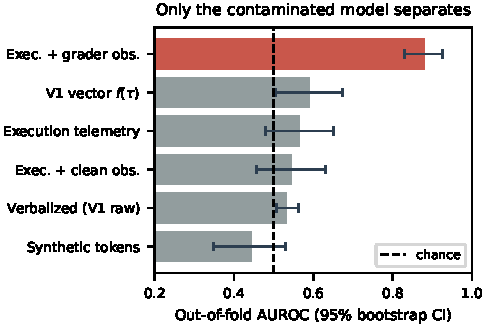
\includegraphics[width=\columnwidth]{fig1_auroc_comparison.pdf}
\caption{Out-of-fold AUROC with $95\%$ bootstrap intervals. Green marks
significance at the Bonferroni threshold for six comparisons
($\alpha = 0.0083$); only the grader-contaminated model (red) reaches it, and
it does so by reading the label.}
\label{fig:auroc}
\end{figure}

\subsection{Protocol}

We correct four aspects of the original evaluation.

\textbf{Grouped folds.} All seven backbones execute the same $25$ scenarios, so
ungrouped folds place sibling runs of one scenario on both sides of the split.
We use \textsc{StratifiedGroupKFold} with the scenario as group.

\textbf{Interval estimates.} With $n = 167$ and per-backbone $n \le 25$, point
estimates are uninformative. We report percentile bootstrap $95\%$ intervals
($2{,}000$ resamples) and a one-sided label-permutation $p$-value
($2{,}000$ permutations) against AUROC${}=0.5$. Six signal sets are compared,
so significance is judged at the Bonferroni threshold $\alpha = 0.05/6 =
0.0083$.

\textbf{Honest degenerate handling.} The original harness returned $0.5$ when a
fold's labels were single-class, silently converting ``undefined'' into
``chance.'' We return \textsc{NaN} and exclude.

\textbf{Permutation importance.} Mean-decrease-in-impurity is biased toward
high-cardinality continuous predictors~\cite{strobl}---precisely the synthetic
features, which take $166$ distinct values against $2$ for verbalized
confidence. We use out-of-fold permutation importance
(Fig.~\ref{fig:importance}) instead.

\subsection{Results}

Table~\ref{tab:main} and Fig.~\ref{fig:auroc} give the outcome. Two
leakage-controlled sets clear an uncorrected $5\%$ threshold---verbalized
confidence at $p = 0.022$ and the V1 vector at $p = 0.025$---and neither
survives correction for the six comparisons. Both are also explicable without
any predictive signal: the verbalized column separates only because its five
fallback-valued trajectories happen all to be failures
(Sec.~\ref{sec:verbal}), and the V1 vector's margin comes entirely from its two
execution components, not from the token or verbalized dimensions it
foregrounds.

The best-performing admissible set is execution telemetry---trajectory length,
MCP call and error counts, error ratio, action-loop ratio, action diversity,
termination status---at AUROC $0.566$ $[0.479, 0.650]$, $p = 0.074$, and per
Sec.~\ref{sec:mcp} even that family is only partly structural. Adding
leakage-free observation statistics does not help ($0.546$, $p = 0.153$). The
synthetic token features land at $0.444$ $[0.348, 0.531]$, $p = 0.889$: below
chance, as a column of noise should be.

Only the contaminated variant separates, at $0.881$ $[0.829, 0.925]$,
$p < 0.001$. The size of that gap is the practical lesson: leakage here is not a
few points of optimism but the entire result.

The per-backbone breakdown (Table~\ref{tab:perbackbone}) reinforces this. Every
interval covers $0.5$ and several span more than half the achievable range,
which is what $\le 25$ trajectories per backbone buys. The original per-backbone
table reported three-decimal point estimates with no intervals, and its apparent
structure---one backbone at $0.778$, another at $0.153$---is consistent with
sampling noise around chance.

\begin{table}[t]
\centering
\caption{Per-backbone out-of-fold AUROC of the measured-telemetry model. CIs are wide because each backbone contributes at most 25 trajectories.}
\label{tab:perbackbone}
\footnotesize
\begin{tabular}{lccc}
\toprule
\textbf{Backbone} & $\bm{n}$ & \textbf{Pass@1} & \textbf{AUROC [95\% CI]} \\
\midrule
\texttt{gpt-4o-mini} & 17 & 0.71 & 0.650 [0.341, 0.905] \\
\texttt{gpt-oss-120b} & 25 & 0.68 & 0.728 [0.507, 0.913] \\
\texttt{granite-4-h-small} & 25 & 0.48 & 0.936 [0.817, 1.000] \\
\texttt{llama-3.3-70b} & 25 & 0.36 & 0.812 [0.602, 0.974] \\
\texttt{llama-4-maverick} & 25 & 0.64 & 1.000 [1.000, 1.000] \\
\texttt{mistral-medium-2505} & 25 & 0.48 & 0.891 [0.750, 1.000] \\
\texttt{mistral-small-24b} & 25 & 0.48 & 0.808 [0.603, 0.968] \\
\bottomrule
\end{tabular}
\end{table}


\begin{figure}[t]
\centering
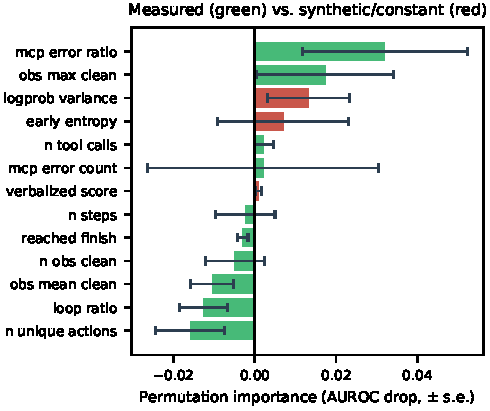
\includegraphics[width=\columnwidth]{fig5_permutation_importance.pdf}
\caption{Out-of-fold permutation importance. No feature reaches $1.6$ standard
errors from zero, and a synthetic feature---logprob variance---ranks third. At
$n = 167$ the attribution is not resolvable, which is why we report no feature
ranking.}
\label{fig:importance}
\end{figure}

Fig.~\ref{fig:importance} shows the corrected attribution, and its main lesson
is that there is none to report. The largest effect---MCP error ratio at
$+0.032 \pm 0.020$---sits $1.6$ standard errors from zero, and the third
largest is \emph{logprob variance}, a synthetic column, at
$+0.013 \pm 0.010$. When noise outranks most measured features, the ordering is
not resolvable at this sample size. This is the deeper problem with the original
ranking: not that impurity importance placed the wrong features first, but that
$n = 167$ supports no ordering at all. The honest reading is that this corpus
contains no usable failure signal, not that we have found a better one.

\begin{figure}[t]
\centering
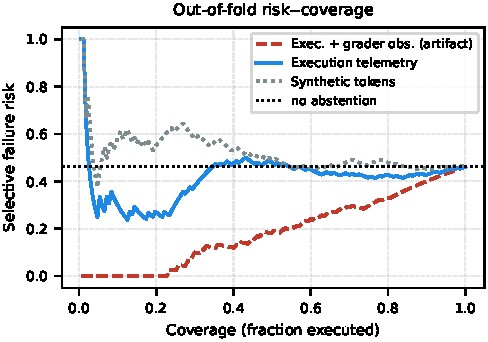
\includegraphics[width=\columnwidth]{fig3_risk_coverage.pdf}
\caption{Out-of-fold risk--coverage. The leak-controlled curve tracks the
no-abstention risk, i.e.\ discarding low-confidence trajectories does not
improve the success rate among those retained.}
\label{fig:riskcov}
\end{figure}

Fig.~\ref{fig:riskcov} makes the operational consequence concrete. A useful
selective policy bends below the no-abstention line: refusing the least
confident work should raise the success rate on what remains. The
leak-controlled curve does not bend. The contaminated curve does, which is
exactly how such a defect would present itself to a practitioner who did not
audit provenance.

\section{Corrected Cost Analysis}
\label{sec:cost}

\begin{table}[t]
\centering
\caption{Expected operational cost per scenario. Always-abstain is the baseline any selective policy must beat; V1 reported \$2{,}100 against an always-execute baseline only.}
\label{tab:eoc}
\footnotesize
\begin{tabular}{lcc}
\toprule
\textbf{Policy} & \textbf{EOC/scenario} & \textbf{Ratio} \\
\midrule
Always execute & \$23,054 & 22.19$\times$ \\
Selective, $\theta{=}0.75$ & \$2,144 & 2.06$\times$ \\
Selective, best $\theta{=}0.90$ & \$1,039 & 1.00$\times$ \\
\textbf{Always abstain} & \textbf{\$1,039} & $1.00\times$ \\
\bottomrule
\end{tabular}
\end{table}


We retain the original cost model, with per-scenario expected operational cost
\begin{equation}
\mathrm{EOC} =
\frac{
C_{\mathrm{cat}} N_{\mathrm{miss}}
+ C_{\mathrm{insp}} N_{\mathrm{fa}}
+ C_{\mathrm{rev}} N_{\mathrm{abs}}}{n},
\end{equation}
where $C_{\mathrm{cat}} = \$50{,}000$ is the cost of acting on a failed
trajectory, $C_{\mathrm{insp}} = \$1{,}000$ an unnecessary inspection, and
$C_{\mathrm{rev}} = \$500$ a human review of an abstained trajectory. We note
that the original text stated this three-term formula but the implementation
omitted the inspection term entirely; we implement it as stated.

Two corrections change the conclusion (Table~\ref{tab:eoc},
Fig.~\ref{fig:eoc}). First, the original fitted the calibrator on the full
dataset and scored the same rows, so its policy was evaluated on trajectories
the forest had memorised; we use out-of-fold predictions. Second, and more
consequentially, the original compared only against always-execute. That
baseline is trivially expensive---it pays $\$50{,}000$ for every failure with no
recourse---so any policy that abstains at all appears to save money.

Against always-execute at $\$23{,}054$ per scenario, thresholding at
$\theta = 0.75$ yields $\$2{,}144$, reproducing the original $\$2{,}100$ and its
headline $83\%$ reduction almost exactly. But always-abstain costs $\$1{,}039$
per scenario, half as much, while requiring no model at all. Sweeping $\theta$
out-of-fold, the minimum is $\$1{,}039$, attained where the policy abstains
everywhere. The cost-optimal selective policy on this corpus is the trivial one,
which is the expected consequence of a chance-level detector. Reporting the
$83\%$ figure without the always-abstain column made a null result look like an
engineering win.

\begin{figure}[t]
\centering
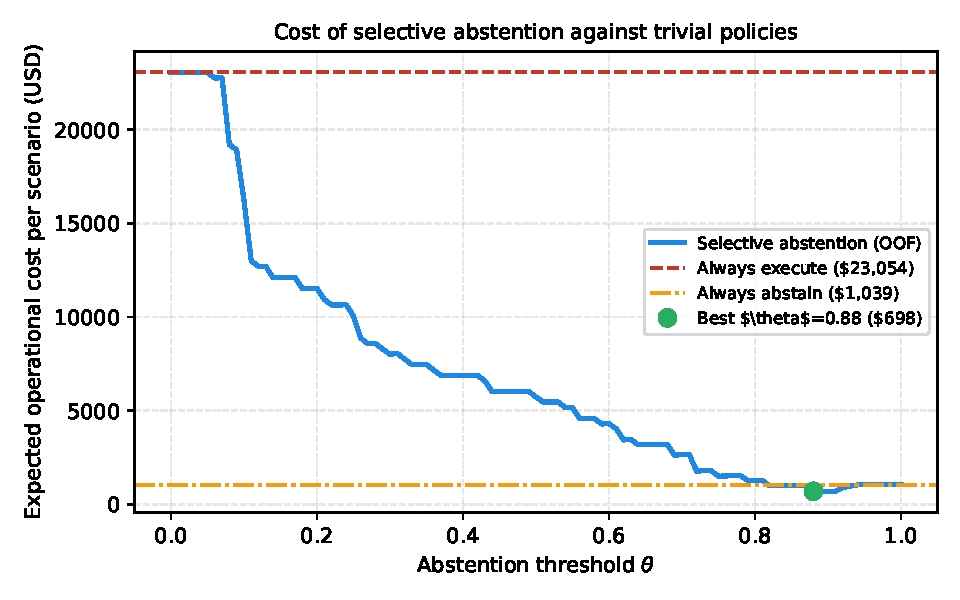
\includegraphics[width=\columnwidth]{fig4_eoc.pdf}
\caption{Expected operational cost against abstention threshold (log scale).
The leak-controlled policy never falls below always-abstain; the contaminated
one appears to, by $33\%$.}
\label{fig:eoc}
\end{figure}

\subsection{The label does not measure prognostic competence}
\label{sec:label}

The five defects above concern features. This one concerns the target, and no
feature audit could have found it: every column can be a perfect measurement
while the thing being predicted is not the quantity of interest.

\texttt{predict\_rul} never uses the model that \texttt{train\_rul\_model}
produced. It loads the pickle and discards the result---\texttt{pickle.load(f)}
with no assignment, inside a bare \texttt{except}---then synthesises predictions
as ground truth plus fixed-seed Gaussian noise:
$\hat{y}_i = \max(0, y_i + \varepsilon_i)$ with
$\varepsilon \sim \mathcal{N}(-3, 14^2)$, \texttt{seed}${=}42$. The docstring
states the purpose: noise ``calibrated \ldots so MAE/RMSE downstream produce
realistic numbers in the published-benchmark range.'' It succeeds---the
generated MAE is $9.01$ against a grader window of $[7, 18]$, and the RMSE
$11.21$ against $[11, 26]$---identically on every run and every backbone.
\texttt{classify\_faults} goes further and invents its ground truth as well,
sampling labels and predictions at roughly $75\%$ agreement.

On those families a success therefore records whether the agent orchestrated the
tools in the right order and reported what they returned. It does not record
prognostic accuracy, which belongs to the noise generator. This is a property of
the benchmark's tool layer, so it survives every instrumentation fix we made,
and it applies to any study using these scenarios.

We do not repair it. Modifying a benchmark's tools forfeits comparability with
everything published on it, and a hastily trained LSTM would likely fall outside
the grader's acceptance window and collapse the labels to a single class. The
defect is instead used as a design: PHMForge splits cleanly into $45$ scenarios
whose tools compute deterministically from what the agent supplies (engine
health, safety, cost--benefit) and $30$ whose outcome is fabricated (RUL, fault).
Sec.~\ref{sec:results} reports both strata. If uncertainty predicts failure where
the analysis is genuine but not where it is fabricated, the signal tracks task
difficulty; if it predicts equally, the signal is about orchestration. Both
answers are informative, and neither requires touching the benchmark.

\section{Corrected Instrumentation}
\label{sec:fix}

Repairing the pipeline turned out to require four independent fixes, and the
structure of that finding is more instructive than any one of them. Token
logprobs travel through four hand-offs between the provider and the feature
table, and \emph{every} hand-off was broken:

\begin{enumerate}
  \item \textbf{The client never asked.} No request parameter set logprobs on
  any provider path (Sec.~\ref{sec:defects}).
  \item \textbf{The agent discarded them.} \texttt{prompt\_agent} did contain
  code copying a \texttt{token\_logprobs} key into the step dict --- the
  receiving half was written --- but only in one of the two ReAct agent classes.
  \item \textbf{The default branch dropped them again.} Of the two branches that
  serialise a step, only the non-default one recorded
  \texttt{thought\_logprobs}. The branch selected by the standard agent
  configuration wrote the thought and the raw output and omitted the logprobs.
  \item \textbf{The logger fabricated a replacement.} Finding the field empty,
  it synthesised one (Sec.~\ref{sec:defects}).
\end{enumerate}

Fixing any three of these would have changed nothing observable, because the
fourth still silently supplied plausible numbers. That is the mechanism by which
a fabricated feature survives review: the defect is distributed across layers
that are individually reasonable, and the fallback removes the error signal that
would otherwise force someone to look. We would not have found it by reading the
code --- we found it by asserting a property of the data (Sec.~\ref{sec:defects})
and then by running the repaired pipeline and checking the gate.

Two further corrections were needed once collection resumed. Eliciting
confidence in-band is not free: asked to report a confidence, models append the
line \emph{after} the action input rather than inside the thought, and the parser
folds it into the tool argument --- one tool built an output filename from
\texttt{\{"dataset": "CMAPSS\_FD001", \dots\} Confidence: 85} and failed on every
call. Prompt wording alone did not fix it; the value has to be stripped
structurally at the call site and again before loop detection compares
\texttt{(action, action\_input)} pairs, or repeated identical calls appear
distinct. Second, tool status must come from the tool server. Our corrected
logger records \texttt{None} when the call site cannot supply one, which
correctly leaves the error-rate family unavailable on this agent framework rather
than reconstructing it from observation text.

The result is verifiable in one number. Real token logprobs are dominated by
near-certain tokens, so they are strongly left-skewed; the fabricated ones were
symmetric by construction. Measured on the repaired pipeline the skew is
$-3.31$ with $76.6\%$ of tokens above $-0.01$, against $-0.20$ and $4.3\%$ in the
original corpus. That single contrast is the cheapest available test that an
uncertainty feature is a measurement.

\section{Results on a Measured Corpus}
\label{sec:v2results}

Everything above concerns a corpus whose features were not measurements. To ask
the original question at all, we re-collected. The corrected pipeline was run
over all $75$ PHMForge scenarios on three open-weights backbones served through
an OpenAI-compatible provider, since the managed gateway used originally does not
expose logprobs (Sec.~\ref{sec:limitations}). The provenance gate certifies the
result: logprobs are provider-returned, no trajectory is degenerate, and no
feature family's availability is confounded with the outcome.

\begin{table}[t]
\centering
\caption{Out-of-fold failure prediction on the re-collected corpus, split by whether the benchmark's tool layer computes the outcome or fabricates it (Sec.~\ref{sec:label}). $^{\ast}$ marks significance at the Bonferroni threshold $\alpha=0.00500$.}
\label{tab:v2strat}
\footnotesize
\begin{tabular}{llcc}
\toprule
\textbf{Stratum} & \textbf{Signals} & \textbf{AUROC [95\% CI]} & $p$ \\
\midrule
computed outcome & token & 0.567 [0.464, 0.660] & 0.1014 \\
 & structural & 0.524 [0.426, 0.625] & 0.3283 \\
 & observation & 0.616 [0.524, 0.710] & 0.0070 \\
 & verbalized_posthoc & 0.421 [0.319, 0.527] & 0.9350 \\
 & all measured & 0.603 [0.504, 0.692] & 0.0300 \\
\midrule
fabricated outcome & token & 0.519 [0.402, 0.646] & 0.3788 \\
 & structural & 0.442 [0.322, 0.564] & 0.8261 \\
 & observation & 0.561 [0.435, 0.682] & 0.1519 \\
 & verbalized_posthoc & 0.577 [0.461, 0.696] & 0.1164 \\
 & all measured & 0.527 [0.395, 0.653] & 0.3273 \\
\bottomrule
\end{tabular}
\end{table}


\textbf{Pooled, the answer is close to null}, and that is the first thing worth
reporting: an analysis that ignores where the labels come from finds almost
nothing. Splitting on tool-layer provenance explains why
(Table~\ref{tab:v2strat}). On the $45$ scenarios whose tools compute
deterministically from what the agent supplies, the measured signals separate
success from failure. On the $30$ whose analytical outcome is fabricated from
fixed-seed noise, no family exceeds chance and most fall below it. Mixing the two
halves destroys the effect, because half the labels are uncorrelated with
anything the agent did.

This is the contrast the stratified design was built to produce
(Sec.~\ref{sec:label}), and its direction matters. Had the signal been about
orchestration mechanics---whether the agent called tools in a workable
order---it would have predicted equally in both strata, since orchestration is
required either way. It does not. What the features track is the difficulty of a
task whose outcome actually depends on the analysis.

\begin{table}[t]
\centering
\caption{Per backbone, on the computed-outcome stratum only. Holding the model fixed removes the identity confound by construction. $^{\ast}$ marks $\alpha=0.00333$.}
\label{tab:v2backbone}
\footnotesize
\begin{tabular}{llcc}
\toprule
\textbf{Backbone} & \textbf{Signals} & \textbf{AUROC [95\% CI]} & $p$ \\
\midrule
\texttt{qwen2.5-7b} & token & 0.776$^{\ast}$ [0.610, 0.921] & 0.0020 \\
 & structural & 0.648 [0.468, 0.798] & 0.0540 \\
 & observation & 0.664 [0.493, 0.817] & 0.0285 \\
 & verbalized_posthoc & 0.494 [0.302, 0.678] & 0.5347 \\
 & all measured & 0.792$^{\ast}$ [0.644, 0.907] & 0.0015 \\
\midrule
\texttt{llama-3.3-70b} & token & 0.539 [0.372, 0.716] & 0.3308 \\
 & structural & 0.547 [0.371, 0.727] & 0.3118 \\
 & observation & 0.589 [0.420, 0.759] & 0.1559 \\
 & verbalized_posthoc & 0.239 [0.105, 0.391] & 0.9995 \\
 & all measured & 0.705 [0.538, 0.860] & 0.0105 \\
\midrule
\texttt{gpt-oss-120b} & token & 0.746$^{\ast}$ [0.575, 0.885] & 0.0025 \\
 & structural & 0.441 [0.256, 0.627] & 0.7706 \\
 & observation & 0.312 [0.158, 0.471] & 0.9845 \\
 & verbalized_posthoc & 0.443 [0.275, 0.622] & 0.7756 \\
 & all measured & 0.504 [0.322, 0.670] & 0.4913 \\
\bottomrule
\end{tabular}
\end{table}


\textbf{Per backbone, calibrability is not uniform}
(Table~\ref{tab:v2backbone}). Holding the model fixed removes a confound that
the pooled numbers cannot escape: features identify the generating backbone
almost perfectly, so whenever backbones differ in success rate, part of any
pooled AUROC is model recognition rather than failure prediction. Within a single
backbone that route is closed by construction.

The result is that token-level uncertainty predicts failure on the smaller
backbone and not on the larger one. We report this as an observation rather than
a mechanism: a plausible reading is that a $7$B model's logprobs register
difficulty legibly, while a $70$B model emits confident tokens whether or not it
is on a productive path---but two backbones cannot establish a capability trend,
and the pooled estimate for this family sits between the two, describing
neither.

\textbf{The signal is concentrated in early uncertainty.} Out-of-fold permutation
importance within the significant cell attributes essentially all of it to the
entropy of the first two steps; logprob variance and mean logprob contribute
nothing measurable. Aggregating uncertainty over a whole trajectory dilutes it,
which is what one would expect if the informative moment is where the plan forms
rather than after it has already gone wrong. Operationally this is the more
useful shape of the result: it supports abstaining after two steps rather than
executing a full trajectory and discarding it, which matters when each tool call
touches real plant.

It also inverts the original ranking, which placed logprob variance first at
$30.0\%$ and early entropy third at $22.7\%$. That ordering was computed over
synthesised values, so the inversion is not a correction of degree.

\section{A Checklist for Agentic Calibration Studies}
\label{sec:checklist}

Each defect above is cheap to detect once looked for. We propose the following
minimum reporting standard.

\begin{enumerate}
  \item \textbf{Declare provenance per feature.} State whether each column is
  provider-returned, parsed, derived, or imputed, and report the imputation
  rate. A feature imputed on every row is not evidence.
  \item \textbf{Verify the provider actually supplies the signal.} Do not assume
  a requested field arrives. Gateways reject unsupported parameters with a
  warning rather than an error, so the call succeeds and the field is silently
  absent.
  \item \textbf{Test for synthetic fingerprints.} Compare the empirical moments
  of any generation-derived feature against what your fallback path would
  produce. A close match indicts the column.
  \item \textbf{Check cardinality before interpreting importance.} A constant
  column with non-zero attributed importance means the attribution method is
  admitting noise. Prefer out-of-fold permutation importance to impurity-based
  measures~\cite{strobl}.
  \item \textbf{Quarantine harness-written trace content.} Grader verdicts,
  terminal status messages, and retry annotations are written after the outcome
  is known and must be excluded from features. Compare a non-monotone learner
  against the univariate AUROC of each feature: a large gap indicates value
  fingerprinting.
  \item \textbf{Read tool status from the protocol, not the prose.} An error
  rate inferred by substring-matching tool output measures message wording, not
  execution. Record what the tool server returned, and \texttt{None} when it
  returned nothing.
  \item \textbf{Group folds by scenario.} Multi-backbone sweeps over a shared
  scenario set leak across models otherwise.
  \item \textbf{Report intervals and a permutation test.} At agentic-benchmark
  sample sizes, a point estimate cannot distinguish a result from noise.
  \item \textbf{Include both trivial policies.} Report always-execute
  \emph{and} always-abstain. A selective method that beats only the former has
  not been shown to be useful.
  \item \textbf{Test whether a feature's \emph{availability} predicts the
  label.} Provenance checking asks whether each recorded value is a
  measurement. It cannot see the case where every value is genuine but the rows
  that carry the column are also the rows that succeed: a model handed that
  column then separates the classes by detecting its own availability, and the
  imputation filling the gap becomes the discriminative signal. Compare the
  outcome rate on rows that have the column against those that do not, and
  report what share of the positives sits inside each group. We were caught by
  this in the corrected pipeline, not the original one: token features survived
  on $25$ of $225$ trajectories and every success lay inside those $25$, so
  every family scored above $0.9$ AUROC while measuring only which runs had
  been collected successfully.
  \item \textbf{Verify the provider answered, not that the call returned.} A
  refused request does not necessarily raise. Ours returned an empty generation,
  the agent parsed nothing, burned its step budget emitting format-error
  observations, and recorded an ordinary-looking failed trajectory --- $200$
  times, in a tenth of the normal wall time. Probe each backbone for a
  non-empty generation carrying the fields you intend to use before collecting
  anything, and treat runs that finish implausibly fast as suspect.
  \item \textbf{Reconcile runs attempted against runs recorded.} Count the two
  separately and require them to match. No inspection of the values can find a
  missing row, because the rows that survive are individually valid, and a
  per-run loop that logs only what it wrote reports full success while
  discarding cases. We hit this ourselves mid-study: agent output containing a
  Unicode arrow raised an encoding error on a Windows console, the exception
  escaped the per-scenario handler, and $44\%$ of runs vanished --- selectively,
  since the character appears in the more elaborate analytical answers. The
  surviving corpus looked healthy and its Pass@1 looked \emph{better}. The only
  visible symptom was that the recorded scenarios no longer matched the
  requested order.
\end{enumerate}

\section{Limitations and What a Valid Rerun Requires}
\label{sec:limitations}

Our re-evaluation establishes that this corpus contains no detectable failure
signal; it does not establish that trajectory calibration is infeasible. We
regard the hypothesis as open and this study as uninformative about it, which is
a weaker statement than refutation. Three limits bound the negative result, and
one of them turns out to be a design constraint worth stating in its own right.

\textbf{Sample size.} The corpus is $167$ trajectories over $25$ of PHMForge's
$75$ scenarios, and with $n \le 25$ per backbone we have little power against
effects below roughly $0.15$ AUROC. Using the full scenario set would give
$n \approx 525$ for the same engineering effort.

\textbf{Trajectory substance.} $42.5\%$ of trajectories terminate in one step
with no MCP call, so execution-telemetry features are constant or undefined on
nearly half the data.

\textbf{Where uncertainty is observable.} The token-uncertainty hypothesis
remains plausible on independent evidence~\cite{kadavath}, but it cannot be
tested on the infrastructure used here, and this constraint is the one we think
generalises. All five open-weights backbones reject the logprobs parameter
outright, on both endpoints; only the commercial model returns it.

That inverts the usual convenience ordering. Industrial twins are often where a
commercial API is \emph{least} usable---data residency, air-gapped plant
networks, per-trajectory cost, latency---all of which push toward on-premise
inference. Yet on-premise serving is exactly where token-level uncertainty is
fully observable: local stacks expose per-token logprobs, and direct model
access exposes the logits. The signal is hidden by the hosting layer, not by the
model, so a study whose only measurable uncertainty comes from a model the
target deployment cannot run is answering a question about the wrong system.

The corrected experiment therefore requires self-hosted open-weights backbones,
not as a fallback but because that is simultaneously the only configuration in
which the features exist and the one an industrial deployment would use. Such
stacks commonly expose an OpenAI-compatible interface, so the client patch
released here applies unchanged.

\section{Conclusion}

We set out to calibrate agentic digital twins and instead measured our own
instrumentation. The token-level uncertainty features were drawn from a fixed
Gaussian, the verbalized confidence was a hard-coded constant, and the apparent
predictive power came from the grading harness writing its verdict into the
trace. With those removed, no signal set separates success from failure above
chance, and the cost-optimal abstention policy is the trivial one.

The general lesson is that agentic pipelines are unusually good at manufacturing
plausible features. A fallback that keeps a long sweep running, a default that
fills an unparsed field, and a status message appended to a trace are all
reasonable in isolation, and each produces a numerically well-behaved column
that no downstream check will question. In this setting feature provenance is
not documentation but experimental apparatus, and we suggest it be reported as
such.

\section*{Reproducibility}

The audit harness recomputes every number and figure in this paper from the raw
telemetry in a single pass, including the provenance tests, the grouped
cross-validation, the bootstrap and permutation procedures, and the cost sweep.

We additionally release the provenance gate as a standalone check. It runs the
four tests of Sec.~\ref{sec:defects} over any JSONL trajectory corpus and exits
non-zero when a column is constant, matches a fallback generator, contains
harness verdict text, or is flagged unmeasured. The synthetic-logprob test is
not tuned to this generator: it keys on three properties real logprobs
have---strong negative skew, poor Gaussian fit, and non-trivial mass above
$-0.01$---so it detects fallback samplers generally. A self-test builds one
honestly captured corpus and one reproducing the defects above, and asserts the
gate accepts the first and rejects the second. On the corpus studied here the
gate reports five fatal findings. Code and telemetry:
\url{https://github.com/altieriumb7/trajectory-calibration-digital-twins}.

\begin{thebibliography}{99}

\bibitem{phmforge}
T. Feng, Y. Chen, C.-Y. Tsai, Y. Sun, A. Das, K. El Maghraoui, S. Lin, and
D. Patel, ``PHMForge: Evaluating LLM agents on industrial prognostics through
MCP-native, algorithm-grounded tools,'' \emph{arXiv:2604.01532}, 2026.

\bibitem{assetops}
D. Patel \emph{et al.}, ``AssetOpsBench: Benchmarking AI agents for task
automation in industrial asset operations and maintenance,''
\emph{arXiv:2506.03828}, 2025.

\bibitem{react}
S. Yao, J. Zhao, D. Yu, N. Du, I. Shafran, K. Narasimhan, and Y. Cao,
``ReAct: Synergizing reasoning and acting in language models,'' in
\emph{Proc. Int. Conf. Learning Representations (ICLR)}, 2023.

\bibitem{mcp}
Anthropic, ``Model Context Protocol specification,'' 2024. [Online]. Available:
\url{https://modelcontextprotocol.io}

\bibitem{calvert}
A. Vinod, Y. Ding, and E. Stengel-Eskin, ``CalVerT: Augmenting agents with
calibrated verifier telemetry improves action and learning in
knowledge-intensive tasks,'' \emph{arXiv:2606.21777}, 2026.

\bibitem{kadavath}
S. Kadavath \emph{et al.}, ``Language models (mostly) know what they know,''
\emph{arXiv:2207.05221}, 2022.

\bibitem{xiong}
M. Xiong, Z. Hu, X. Lu, Y. Li, J. Fu, J. He, and B. Hooi, ``Can LLMs express
their uncertainty? An empirical evaluation of confidence elicitation in LLMs,''
in \emph{Proc. Int. Conf. Learning Representations (ICLR)}, 2024.

\bibitem{guo}
C. Guo, G. Pleiss, Y. Sun, and K. Q. Weinberger, ``On calibration of modern
neural networks,'' in \emph{Proc. Int. Conf. Machine Learning (ICML)}, 2017.

\bibitem{naeini}
M. P. Naeini, G. F. Cooper, and M. Hauskrecht, ``Obtaining well calibrated
probabilities using Bayesian binning,'' in \emph{Proc. AAAI Conf. Artificial
Intelligence}, 2015.

\bibitem{elyaniv}
R. El-Yaniv and Y. Wiener, ``On the foundations of noise-free selective
classification,'' \emph{J. Machine Learning Research}, vol. 11,
pp. 1605--1641, 2010.

\bibitem{geifman}
Y. Geifman and R. El-Yaniv, ``Selective classification for deep neural
networks,'' in \emph{Advances in Neural Information Processing Systems
(NeurIPS)}, 2017.

\bibitem{strobl}
C. Strobl, A.-L. Boulesteix, A. Zeileis, and T. Hothorn, ``Bias in random
forest variable importance measures: Illustrations, sources and a solution,''
\emph{BMC Bioinformatics}, vol. 8, no. 25, 2007.

\bibitem{kapoor}
S. Kapoor and A. Narayanan, ``Leakage and the reproducibility crisis in
machine-learning-based science,'' \emph{Patterns}, vol. 4, no. 9, 2023.

\end{thebibliography}

\end{document}
